\documentclass[border=2pt]{standalone}
\usepackage[dvipsnames,svgnames,x11names]{xcolor}
\usepackage{tikz}
\usetikzlibrary{arrows.meta,backgrounds,fit}
\begin{document}
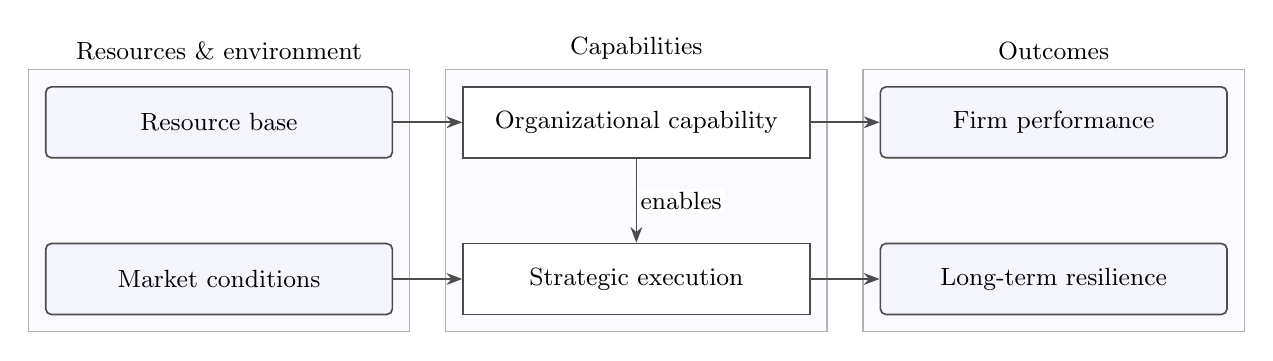
\begin{tikzpicture}[font=\small,>=Stealth,x=53.0mm,y=19.9mm]
\node[rectangle,rounded corners=2pt,fill=blue!4,draw=black!70,text=black,line width=0.6pt,minimum height=9mm,inner xsep=7pt,inner ysep=4.5pt,align=center,text width=39.1mm,execute at begin node={\hyphenpenalty=10000\relax}] (r1) at (0,0) {Resource base};
\node[rectangle,rounded corners=2pt,fill=blue!4,draw=black!70,text=black,line width=0.6pt,minimum height=9mm,inner xsep=7pt,inner ysep=4.5pt,align=center,text width=39.1mm,execute at begin node={\hyphenpenalty=10000\relax}] (r2) at (0,-1) {Market conditions};
\node[rectangle,fill=white,draw=black!70,text=black,line width=0.6pt,minimum height=9mm,inner xsep=7pt,inner ysep=4.5pt,align=center,text width=39.1mm,execute at begin node={\hyphenpenalty=10000\relax}] (c1) at (1,0) {Organizational capability};
\node[rectangle,fill=white,draw=black!70,text=black,line width=0.6pt,minimum height=9mm,inner xsep=7pt,inner ysep=4.5pt,align=center,text width=39.1mm,execute at begin node={\hyphenpenalty=10000\relax}] (c2) at (1,-1) {Strategic execution};
\node[rectangle,rounded corners=2pt,fill=blue!4,draw=black!70,text=black,line width=0.6pt,minimum height=9mm,inner xsep=7pt,inner ysep=4.5pt,align=center,text width=39.1mm,execute at begin node={\hyphenpenalty=10000\relax}] (p1) at (2,0) {Firm performance};
\node[rectangle,rounded corners=2pt,fill=blue!4,draw=black!70,text=black,line width=0.6pt,minimum height=9mm,inner xsep=7pt,inner ysep=4.5pt,align=center,text width=39.1mm,execute at begin node={\hyphenpenalty=10000\relax}] (p2) at (2,-1) {Long-term resilience};
\begin{scope}[on background layer]
\node[fit=(r1)(r2),inner sep=6pt,fill=blue!2,draw=black!30,line width=0.45pt,label={[font=\small]above:{Resources \& environment}}] (inputs) {};
\node[fit=(c1)(c2),inner sep=6pt,fill=blue!2,draw=black!30,line width=0.45pt,label={[font=\small]above:{Capabilities}}] (capabilities) {};
\node[fit=(p1)(p2),inner sep=6pt,fill=blue!2,draw=black!30,line width=0.45pt,label={[font=\small]above:{Outcomes}}] (performance) {};
\end{scope}
\draw[->,draw=black!70,line width=0.6pt] (r1) -- (c1);
\draw[->,draw=black!70,line width=0.6pt] (r2) -- (c2);
\draw[->,draw=black!70,line width=0.6pt] (c1) -- (p1);
\draw[->,draw=black!70,line width=0.6pt] (c2) -- (p2);
\draw[->,draw=black!70,line width=0.6pt] (c1) -- node[pos=0.5,right,fill=white,inner sep=1.2pt] {enables} (c2);
\end{tikzpicture}
\end{document}
